\documentclass[11pt,a4paper]{article}

\usepackage[T1]{fontenc}
\usepackage[utf8]{inputenc}
\usepackage{mathpazo}
\usepackage[margin=2.2cm]{geometry}
\usepackage{booktabs,tabularx,array,multirow}
\usepackage{graphicx}
\usepackage{caption}
\usepackage{enumitem}
\usepackage{amssymb}
\usepackage{xcolor}
\usepackage{fancyhdr}
\usepackage[colorlinks=true,linkcolor=blue!50!black,urlcolor=blue!50!black]{hyperref}

\newcommand{\teamname}{Project 5}
\newcommand{\projecttitle}{Camera-Trap Image Classification}

\newcommand{\prompt}[1]{\leavevmode{\color{gray!80!black}\itshape #1}}
\newcommand{\blank}{\rule{0pt}{2.2ex}}
\newcommand{\pts}[1]{\texorpdfstring{\hfill{\normalsize\mdseries(#1 points)}}{}}
\newlist{checklist}{itemize}{1}
\setlist[checklist]{label=$\square$,leftmargin=1.6em,itemsep=2pt}
\newcolumntype{Y}{>{\raggedright\arraybackslash}X}
\renewcommand{\arraystretch}{1.25}
\setlength{\parindent}{0pt}
\setlength{\parskip}{4pt}
\emergencystretch=2em

\pagestyle{fancy}
\fancyhf{}
\lhead{\itshape AI251P Applied Computer Vision}
\rhead{\itshape Capstone Phase 1 Report -- \teamname}
\cfoot{\thepage}
\setlength{\headheight}{14pt}

\begin{document}

\begin{center}
  {\large AI251P Applied Computer Vision}\\[4pt]
  {\LARGE\bfseries Capstone Project -- Phase 1 Report}\\[6pt]
  {\Large \projecttitle}\\[4pt]
  \teamname\ \textperiodcentered\ Phase 1 (M1--M3, 40 points) \textperiodcentered\ Due 28 October 2026
\end{center}
\vspace{4pt}

\section{Team and project}

\begin{tabularx}{\linewidth}{@{}l Y@{}}
\toprule
Field & Description \\
\midrule
Team name & Project 5 \\
Topic & Project 5: camera-trap image classification \\
Application area & Wildlife monitoring and image triage \\
Code repository & \url{https://github.com/salehdev3/Capstone_5} \\
W\&B project & \url{https://wandb.ai/saleh-alanazi-ministry-of-interior/camera-trap-phase1} \\
Dataset card & \url{https://github.com/salehdev3/Capstone_5/blob/v1/DATASET_CARD.md} \\
\bottomrule
\end{tabularx}

\subsection*{Team members}

\begin{tabularx}{\linewidth}{@{}l l l Y@{}}
\toprule
Name & Student ID & Workstream (Table 3) & Phase 1 contribution \\
\midrule
Saud Abdullah Alfaiz & 225462 & Data and classification & Data preparation, grouped split, audit and card \\
Saleh Mohammed Alanazi & 225486 & Data and classification & Scratch CNN and evaluation \\
Yousef Nafi Alanazi & 225457 & Data and classification & Frozen and full ResNet-50 comparison \\
Mohannad Mohammed Alqahtani & 225461 & Integration & Independent review, comparison and report \\
\bottomrule
\end{tabularx}

\subsection*{Problem and acceptance criteria}

\begin{itemize}[leftmargin=1.2em]
  \item \textbf{Summary:} The system classifies full camera-trap frames as empty or animal, then predicts animal species on human-box crops. It reports per-class metrics, calibration and errors.
  \item \textbf{Input $\rightarrow$ output:} A camera-trap photograph $\rightarrow$ empty/animal decision; an annotated animal crop $\rightarrow$ species category.
  \item \textbf{Intended users and the decision supported:} Wildlife-data reviewers use it to prioritize animal frames and inspect species predictions.
  \item \textbf{Acceptance criteria (fixed before results):} Animal recall $\geq .99$; empty removal $\geq .20$; species macro-F1 $\geq .65$; species ECE $\leq .10$.
\end{itemize}

\section{Data foundations (M1)\pts{12}}

\subsection{Datasets}

{\small
\begin{tabularx}{\linewidth}{@{}l l Y l l r@{}}
\toprule
Dataset & Link / ref. & Content and annotations & Use & Licence & Images \\
\midrule
CCT20 subset & LILA CCT & Camera-trap frames and human boxes & All splits & CDLA-Permissive & 6,022 \\
Team frames & Local collection & Reviewed frames and boxes & Train/test & Team-owned & 19 \\
\bottomrule
\end{tabularx}}

\smallskip
The notebook selected 6,022 CCT20 images under a fixed seed of 42, then included 19 reviewed team images. This project-specific subset does not use the official CCT benchmark split.

\subsection{Cleaning}

\begin{tabularx}{\linewidth}{@{}l Y r@{}}
\toprule
Check & Method / tool & Images removed \\
\midrule
Corrupt or unreadable files & Download/decode checks & 0 \\
Exact duplicates & ID/hash checks & 0 \\
Near-duplicates & pHash cross-partition checks & 0 \\
Other (human audit quarantine) & One flagged event, four frames & 4 \\
\midrule
\textbf{Images remaining} & 6,041 initially kept; 6,037 after audit & 6,037 \\
\bottomrule
\end{tabularx}

\subsection{Leakage-safe split}

\begin{itemize}[leftmargin=1.2em]
  \item \textbf{Grouping key:} CCT20 camera/event; local images by city and session.
  \item \textbf{Why this prevents leakage:} Frames from the same camera or burst share backgrounds, lighting and animals; grouping keeps these correlations within one partition.
  \item \textbf{Stratification and seed:} Group-aware approximate joint-label stratification, seed 42. Camera separation takes priority over exact class proportions.
\end{itemize}

\begin{tabularx}{\linewidth}{@{}l r r Y@{}}
\toprule
Split & No. of Groups & No. of Images & Images per class (or \% of the smallest class) \\
\midrule
Train & 13 & 3,534 & Empty: 319; animal: 3,215 \\
Validation selection & 3 & 1,337 & Empty: 91; animal: 1,246 \\
Validation calibration & 2 & 527 & Empty: 13; animal: 514 \\
Test & 4 & 639 & Empty: 53; animal: 586 \\
\bottomrule
\end{tabularx}

\subsection{Species crop support by split}

\begin{center}
{\small
\begin{tabular}{lrrrr}
\toprule
Species & Train & Selection & Calibration & Test \\
\midrule
Badger & 4 (0.1\%) & 0 (0.0\%) & 0 (0.0\%) & 1 (0.2\%) \\
Bird & 116 (4.1\%) & 3 (0.3\%) & 45 (9.3\%) & 9 (1.8\%) \\
Bobcat & 286 (10.1\%) & 25 (2.2\%) & 78 (16.1\%) & 57 (11.2\%) \\
Cat & 142 (5.0\%) & 247 (22.0\%) & 35 (7.2\%) & 48 (9.4\%) \\
Coyote & 288 (10.2\%) & 29 (2.6\%) & 37 (7.7\%) & 169 (33.3\%) \\
Deer & 11 (0.4\%) & 0 (0.0\%) & 0 (0.0\%) & 3 (0.6\%) \\
Dog & 117 (4.2\%) & 33 (2.9\%) & 73 (15.1\%) & 29 (5.7\%) \\
Fox & 1 (0.0\%) & 0 (0.0\%) & 0 (0.0\%) & 1 (0.2\%) \\
Opossum & 622 (22.1\%) & 489 (43.5\%) & 99 (20.5\%) & 87 (17.1\%) \\
Rabbit & 317 (11.2\%) & 164 (14.6\%) & 61 (12.6\%) & 4 (0.8\%) \\
Raccoon & 709 (25.2\%) & 14 (1.2\%) & 28 (5.8\%) & 28 (5.5\%) \\
Rodent & 38 (1.3\%) & 0 (0.0\%) & 0 (0.0\%) & 0 (0.0\%) \\
Skunk & 73 (2.6\%) & 0 (0.0\%) & 21 (4.3\%) & 19 (3.7\%) \\
Squirrel & 95 (3.4\%) & 120 (10.7\%) & 6 (1.2\%) & 53 (10.4\%) \\
\midrule
Total crops & 2,819 (100\%) & 1,124 (100\%) & 483 (100\%) & 508 (100\%) \\
\bottomrule
\end{tabular}}
\end{center}
Each cell gives crop count and percentage of crops in that split. Crop counts differ from frame counts because a frame may contain multiple annotated animals. Species with zero support in a split are shown as zero.

The table reports annotated animal crops, not frame counts. A frame may contain multiple animals. Zero denotes no annotated crop for that species in the corresponding split. The source counts are archived in \texttt{evidence/species\_crop\_support.csv}.

\subsection{Label audit}

\begin{tabularx}{\linewidth}{@{}Y Y Y Y@{}}
\toprule
Audited sample size & Errors found & Estimated label-error rate & Upper bound (95\% confidence) \\
\midrule
10 training events & 1 & 10\% & 39.4\% one-sided \\
\bottomrule
\end{tabularx}

\smallskip
One frame was drawn from each of 10 random training events; the team found one incorrect label and quarantined the affected event. A separate 20-image review signed by Mohannad Mohammed Alqahtani found no additional frame-label errors; five box checks were not applicable.

\subsection{Data loader and augmentation}

RGB images were prepared with maximum side 1,024 pixels, resized to 224$\times$224, then ImageNet-normalized. Training alone uses random flip and brightness/contrast augmentation from the shared preprocessing module; these variations reflect camera viewpoint and illumination. Exact augmentation parameters are fixed in \texttt{preprocessing.py}.

\subsection{Dataset card summary}

Raccoon and opossum dominate some groups while rare species have few examples; camera-group splits have distribution shift. CCT20 is largely US wildlife, and five held-out Tabuk frames cannot establish Saudi deployment performance. The small audit has a wide error bound. Source terms and course policy restrict image redistribution. Team images are tracked in the repository and are subject to the team collection and publication policy. The full card is linked in Section 1.

\section{Classification (M2--M3)\pts{20}}

\textbf{Task:} Full frames are classified empty/animal; human-box crops are classified by species. These classifiers provide the baseline for later detection and segmentation.

\subsection{Runs compared}

Six regimes were compared using validation-selection macro-F1; frozen ResNet-50 was chosen for both tasks. The locked test set was evaluated after selection. W\&B links for all six runs are in the linked project.

\medskip
{\small
\begin{tabularx}{\linewidth}{@{}l l Y r r r r@{}}
\toprule
Run (W\&B link) & Backbone & Training & Input res. & Epochs & Val.\ acc. & Val.\ macro-F1 \\
\midrule
Triage (W\&B) & CNN & From scratch & 224 & 6 & .941 & .601 \\
Triage (W\&B) & ResNet-50 & Pretrained, frozen & 224 & 12 & .940 & .662 \\
Triage (W\&B) & ResNet-50 & Pretrained, full fine-tuning & 224 & 12 & .927 & .640 \\
Species (W\&B) & CNN & From scratch & 224 & 12 & .505 & .156 \\
Species (W\&B) & ResNet-50 & Pretrained, frozen & 224 & 12 & .761 & .364 \\
Species (W\&B) & ResNet-50 & Pretrained, full fine-tuning & 224 & 12 & .750 & .340 \\
\bottomrule
\end{tabularx}}

\medskip
\textbf{Test-set results (final models only)}

\smallskip
\begin{tabularx}{\linewidth}{@{}Y r r r@{}}
\toprule
Run & Test accuracy (95\% CI) & Test macro-F1 & ECE \\
\midrule
Triage scratch & .917 [.868,.966] & .478 & .0463 \\
Triage frozen (selected) & .933 [.897,.967] & .652 & .0460 \\
Species scratch & .350 [.284,.386] & .178 & .0733 \\
Species frozen (selected) & .742 [.642,.876] & .482 & .0568 \\
\bottomrule
\end{tabularx}

\smallskip
\textbf{Which model you keep and why:} Frozen ResNet-50 gave the highest validation macro-F1 for both tasks (.662 triage and .364 species). It was therefore retained before test results were examined. At test threshold .3416, triage retained 586/586 animal frames but removed only 6/53 empty frames (11.3\%), missing the 20\% empty-removal target. Species test macro-F1 was .482, below the .65 target; ECE .0568 met the .10 limit.

All accuracy and per-class tables above use argmax. The separate operating policy uses animal probability $\geq 0.3416247$, selected on \texttt{val\_calibrate} to maximize empty removal subject to empirical animal recall $\geq .99$. Calibration retained 509/514 animals and removed 2/13 empty frames. This empirical constraint is not a population guarantee.

Accuracy intervals are 2.5th--97.5th percentile camera-cluster bootstrap intervals (1,000 resamples, seed 42), resampling whole cameras with replacement. Only four test groups are available; intervals are descriptive and unstable. They are not independent-image confidence intervals.

Species macro-F1 is .481994 across all 14 training classes, and .519070 across the 13 classes with test support. Rodent has zero test examples. Both definitions are retained; excluding the unsupported class does not indicate model improvement.

The held-out Tabuk subset contains five frames and overlaps the combined test. Saved per-camera argmax accuracy is 2/5 for triage and 4/5 for species. This small, imbalanced subset does not establish deployment performance and is not an additional independent test.

\subsection{Learning curves}

\begin{figure}[htbp]
  \centering
  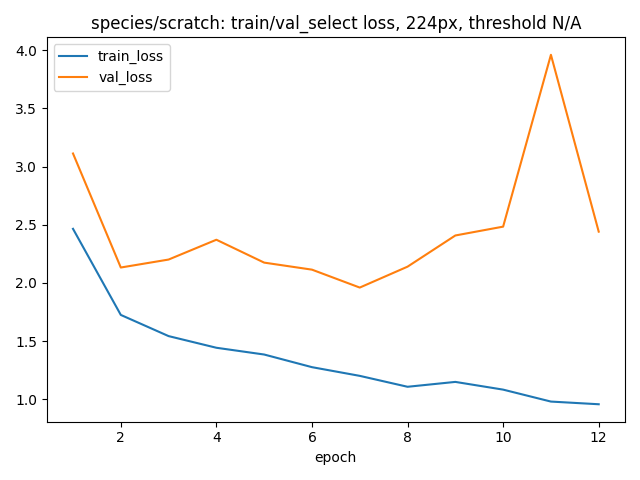
\includegraphics[width=0.48\linewidth]{figures/species_scratch_loss.png}\hfill
  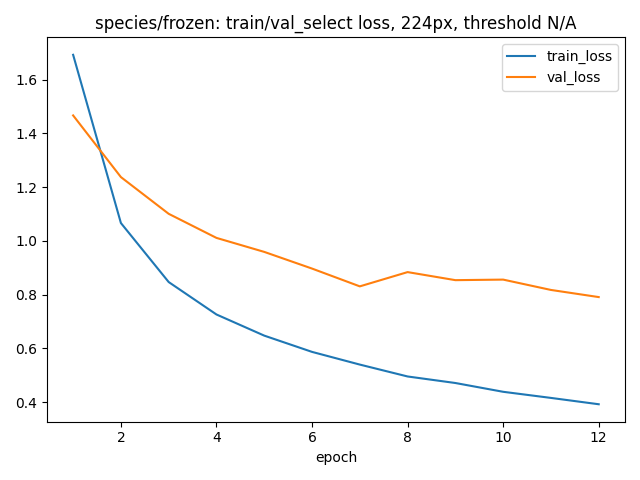
\includegraphics[width=0.48\linewidth]{figures/species_frozen_loss.png}
  \caption{Training and validation-selection loss: (left) scratch CNN, (right) frozen ResNet-50. Split: train and validation-selection; input: 224$\times$224; threshold: argmax.}
\end{figure}

Species full fine-tuning reached 94.7\% training accuracy but 75.0\% validation accuracy, consistent with overfitting. Frozen species reached 89.7\% and 76.1\%, respectively. Rare-class support and camera shift remain important limits.

\subsection{Per-class results (selected model, test set)}

\begin{tabularx}{\linewidth}{@{}Y r r r r@{}}
\toprule
Class & Precision & Recall & F1 & Support \\
\midrule
Empty (triage) & .917 & .208 & .338 & 53 \\
Animal (triage) & .933 & .998 & .965 & 586 \\
\midrule
Badger (species) & .000 & .000 & .000 & 1 \\
Bird (species) & .900 & 1.000 & .947 & 9 \\
Bobcat (species) & .629 & .684 & .655 & 57 \\
Cat (species) & .632 & .250 & .358 & 48 \\
Coyote (species) & .956 & .763 & .849 & 169 \\
Deer (species) & .000 & .000 & .000 & 3 \\
Dog (species) & .676 & .862 & .758 & 29 \\
Fox (species) & .000 & .000 & .000 & 1 \\
Opossum (species) & .656 & .966 & .781 & 87 \\
Rabbit (species) & .250 & .250 & .250 & 4 \\
Raccoon (species) & .366 & .536 & .435 & 28 \\
Rodent (species) & .000 & .000 & .000 & 0 \\
Skunk (species) & .933 & .737 & .824 & 19 \\
Squirrel (species) & .860 & .925 & .891 & 53 \\
\midrule
\textbf{Macro average (species)} & .490 & .498 & .482 & 508 \\
\bottomrule
\end{tabularx}

\smallskip
Top-$k$ accuracy (species, $k=3$): .9055 on test; 224$\times$224, argmax.

\subsection{Triage confusion matrices}
Rows are true labels; columns are predictions. Split: test, input: $224\times224$. These tables use all 639 frames.
\begin{center}
\begin{tabular}{lrr|rr}
\toprule
& \multicolumn{2}{c}{Argmax} & \multicolumn{2}{c}{Threshold .3416247} \\
True label & Empty & Animal & Empty & Animal \\
\midrule
Empty & 11 & 42 & 6 & 47 \\
Animal & 1 & 585 & 0 & 586 \\
\bottomrule
\end{tabular}
\end{center}

\subsection{Confusion matrix and calibration}

\begin{figure}[htbp]
  \centering
  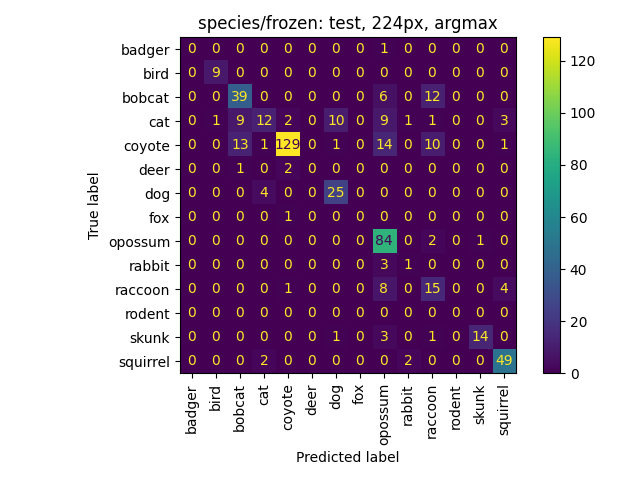
\includegraphics[width=0.48\linewidth]{figures/species_frozen_confusion.png}\hfill
  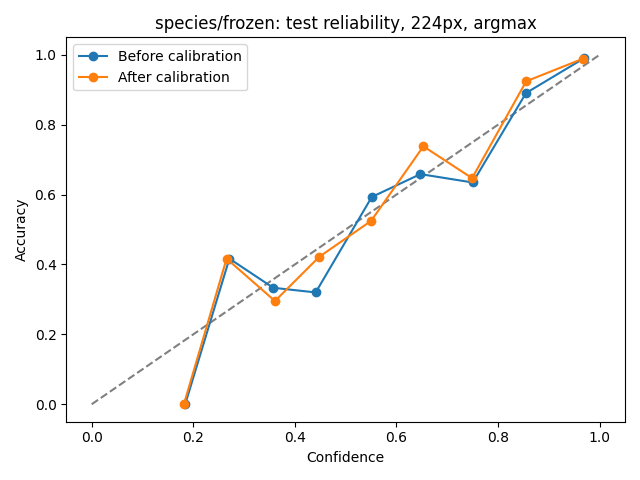
\includegraphics[width=0.48\linewidth]{figures/species_frozen_reliability.png}
  \caption{(Left) confusion matrix; (right) reliability diagram. Split: test; input: 224$\times$224; threshold: argmax.}
\end{figure}

Bobcat was repeatedly confused with raccoon in the gallery; a fox crop was called coyote. Selected species test ECE was .0568 versus raw .0454, so temperature scaling did not improve ECE on this test split. Gallery observations are not a causal proof.

\subsection{Error analysis}

\begin{figure}[htbp]
  \centering
  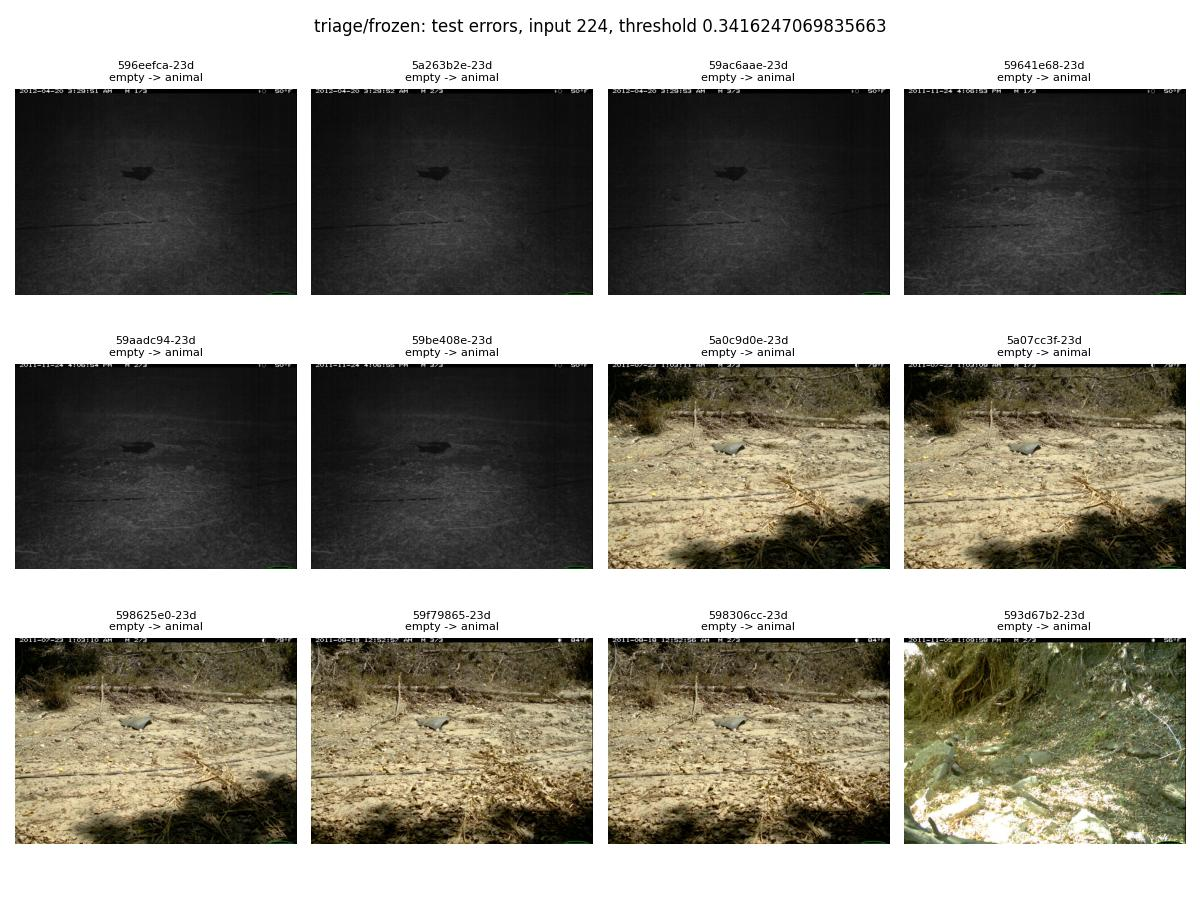
\includegraphics[width=0.9\linewidth]{figures/triage_frozen_errors.jpg}
  \caption{Triage test error gallery: recorded label and prediction are shown; input 224$\times$224, animal threshold .3416. Visual inspection indicates potential source-label ambiguity.}
\end{figure}

\begin{tabularx}{\linewidth}{@{}Y r Y@{}}
\toprule
Error pattern & Full-test count / gallery & Likely cause (data, label, model) \\
\midrule
Recorded empty $\rightarrow$ animal & 47 total; 12 shown & Bird-like visual features in several daylight frames indicate potential source-label ambiguity. \\
Bobcat $\rightarrow$ raccoon & 12 total; 5 shown & Low-detail night crops and camera-domain shift are plausible contributors. \\
\bottomrule
\end{tabularx}

Counts above cover all test decisions: triage uses the calibrated threshold, species uses argmax. Visual explanations are hypotheses, not counts of verified night-time causes.

\subsection{Data-improvement plan}

\begin{tabularx}{\linewidth}{@{}Y Y Y@{}}
\toprule
Finding from the error analysis & Planned action & Expected effect \\
\midrule
Possible source-label errors & Full-resolution annotation review and a separate corrected-label sensitivity analysis & Distinguish annotation issues from model errors \\
Rare species and empty frames & Validation-selection comparison of class-weighted loss and the baseline, with additional independently grouped examples & Measure minority recall and empty removal without tuning on test \\
Low-detail night crops & Full-test illumination annotation and validation-based comparison of night-focused training data and illumination augmentation & Night-time recall and calibration measured against the baseline \\
\bottomrule
\end{tabularx}

\section{Reproducibility\pts{8}}

\begin{tabularx}{\linewidth}{@{}l Y@{}}
\toprule
Item & Description \\
\midrule
Repository and commit hash & \url{https://github.com/salehdev3/Capstone_5}, evaluated results release \texttt{2cc1731} on \texttt{v1} \\
Configuration file used for the reported runs & \texttt{handoff/data\_config.json} and \texttt{runs/member2,member3/config.json} \\
Random seeds & 42 \\
Requirements file (pinned versions) & Pinned CPU validation environment: \texttt{requirements-cpu-validation.txt}. Historical GPU run configurations are recorded in W\&B. \\
Command(s) to reproduce the main result & Run \texttt{notebooks/Phase1\_Final\_Presentation.ipynb} in section order on Colab GPU \\
Data sources & CCT20 on LILA; team photos tracked in the repository; recorded manifest hash in dataset card \\
Reproduction evidence and scope & Fresh-process checkpoint inference is recorded in \texttt{review/fresh\_process\_results.json}. Instructor feedback separately identifies a matching full W\&B rerun on 28 October, attributed by the team to Mohannad. Checkpoint inference and full training replay are reported as distinct validation procedures \\
\bottomrule
\end{tabularx}

\section{Submission checklist}

\begin{checklist}
  \item Corrupt files and duplicates handled, with counts reported
  \item Split is grouped by the source of correlation; the grouping key is justified
  \item Label audit reported with a confidence bound
  \item Dataset card states licences, limitations and privacy measures
  \item Scratch and fine-tuned classifiers compared in W\&B
  \item Per-class metrics, confusion matrix and calibration (ECE) reported
  \item Test set used only for final evaluation, not model selection
  \item Data-improvement plan follows from the error analysis
  \item Fixed seeds, recorded training configuration, and a pinned CPU validation environment
  \item Every figure states split, input resolution and thresholds
  \item Team photos are identified as tracked repository content
\end{checklist}

\section{Self-assessment}

\begin{tabularx}{\linewidth}{@{}l c c Y Y@{}}
\toprule
Criterion & Points & Self-score & Strongest evidence (section) & Known gap \\
\midrule
Data foundations and dataset card (M1) & 12 & 11 & Cleaning, split, audit, card & Small initial audit \\
Classification (M2--M3) & 20 & 19 & Six runs, metrics and galleries & Two preset targets missed \\
Reproducibility & 8 & 6 & Config, hashes, inference check & CPU environment pinning and checkpoint inference are distinct from full GPU replay \\
\midrule
\textbf{Total} & \textbf{40} & \textbf{36} & Instructor Phase 1 feedback & Phase 1 assessment \\
\bottomrule
\end{tabularx}

\section{Obstacles and how they were addressed}

A Colab upload stall interrupted evaluation. The evaluation workflow now saves test metrics before a time-bounded W\&B upload, so a stalled upload does not block the local results.

\medskip
{\small
\begin{tabularx}{\linewidth}{@{}Y l Y Y l@{}}
\toprule
Obstacle & Module & Impact on the work & Action taken & Status \\
\midrule
Colab upload stalls & M2--M3 & Evaluation interruption & Save metrics before bounded W\&B upload & Resolved \\
\bottomrule
\end{tabularx}}


\end{document}
